\documentclass{article}
\usepackage[T1]{fontenc}
\usepackage{lmodern}
\usepackage[polish]{babel}
\usepackage{graphicx}
\usepackage{float}
\usepackage{hyperref}
\usepackage{amsmath}
\usepackage{listings}
\usepackage{xcolor}

\usepackage[a4paper, margin=2.54cm]{geometry}

\title{Praca domowa 6\\Klasyfikator Bayesa oraz K-NN}
\author{Damian Jankowski s188597}

\begin{document}

\maketitle

\section{Wstęp}

Celem pracy domowej było zapoznanie się z klasyfikatorem Bayesa oraz
klasyfikatorem K-NN. W dziedzinie uczenia maszynowego klasyfikatory 
Bayesa i K-NN (k najbliższych sąsiadów) są 
często wykorzystywane do rozwiązywania problemów klasyfikacji. 
Klasyfikator Bayesa jest probabilistycznym modelem, 
który wykorzystuje twierdzenie Bayesa do obliczenia 
prawdopodobieństwa przynależności obserwacji do danej klasy. 
Klasyfikator K-NN natomiast jest modelem, 
który przypisuje nową obserwację do klasy najczęściej 
występującej wśród jej k najbliższych sąsiadów.

\subsection{Klasyfikator Bayesa}
Klasyfikator Bayesa oparty jest na twierdzeniu Bayesa, 
które jest podstawą teorii prawdopodobieństwa. Zakłada 
się, że obserwacje są niezależne i pochodzą z pewnego 
rozkładu prawdopodobieństwa. Klasyfikator Bayesa 
wykorzystuje te informacje, aby obliczyć prawdopodobieństwo 
przynależności danej obserwacji do poszczególnych klas.

Załóżmy, że mamy zbiór danych uczących składający się z 
obserwacji $d$ i odpowiadających im etykiet klas $C$. 
Klasyfikator Bayesa szacuje prawdopodobieństwo warunkowe 
$P(C_i|d)$, czyli prawdopodobieństwo przynależności i-tej
klasy do obserwacji. Wykorzystuje przy tym 
twierdzenie Bayesa, które można zapisać jako:

\begin{equation}
    P(C_i|d) = \frac{P(C_i)P(d|C_i)}{P(d)}
\end{equation}

Po zamianie obserwacji $d$ na wektor cech $w$ otrzymujemy:

\begin{equation}
    P(C_i|w_1, w_2, ..., w_n) = \frac{P(C_i)P(w_1, w_2, ..., w_n|C_i)}{P(w_1, w_2, ..., w_n)}
\end{equation}

co można przedstawić w postaci:

\begin{equation}
    P(C_i|w_1, w_2, ..., w_n) = \frac{P(C_i)\prod_{j=1}^{n}P(w_j|C_i)}{P(w_1, w_2, ..., w_n)}
\end{equation}

gdzie:
\begin{itemize}
    \item $P(C_i)$ - prawdopodobieństwo wystąpienia i-tej klasy, wyrażona jako 
    stosunek liczby obserwacji ze znaną i-tą klasą do liczby wszystkich obserwacji
    należących do $m$ klas:
    $P(C_i) = \cfrac{|C_i|}{\sum_{j=1}^{m}|C_j|}$
    \item $P(w_j|C_i)$ - prawdopodobieństwo wystąpienia j-tej cechy w i-tej klasie,
    wyrażona jako stosunek liczby obserwacji z i-tą klasą, w których występuje j-ta cecha,
    do liczby wszystkich obserwacji z i-tą klasą:
    $P(w_j|C_i) = \cfrac{|w_j, C_i|}{|C|}$
\end{itemize}

\newpage

By uniknąć problemu z zerowymi prawdopodobieństwami,
które mogą wystąpić, gdy na przykład w zbiorze uczącym nie ma obserwacji
z daną cechą, stosuje się wygładzanie Laplace'a. Polega ono
na wyznaczeniu stosunku liczby wystąpień danej cechy w danej klasie
powiększonej o 1, do liczby wszystkich cech w danej klasie powiększonej
o liczbę wszystkich cech w zbiorze uczącym.

\begin{equation}
    P(w_j|C_i) = \cfrac{|w_j, C_i| + 1}{|w, C_i| + |v|}
\end{equation}

Po wyznaczeniu prawdopodobieństw warunkowych $P(C_i|w_1, w_2, ..., w_n)$ dla każdej klasy
$C_i$ klasyfikator Bayesa przypisuje obserwację $d$ do klasy $C_i$, dla której prawdopodobieństwo
warunkowe jest największe (z zasady maksimum a posteriori).

\begin{equation}
    C_{pred} = \arg\max_{i}P(C_i|w_1, w_2, ..., w_n)
\end{equation}

\subsection{Klasyfikator K-NN}

Klasyfikator K-NN przypisuje nową obserwację do klasy najczęściej
występującej wśród jej k najbliższych sąsiadów. W tym celu wykorzystuje
metrykę odległości, która określa odległość między dwoma obserwacjami.
Najczęściej stosowaną metryką jest metryka euklidesowa, która dla dwóch
obserwacji $d_1$ i $d_2$ wyraża się wzorem:

\begin{equation}
    d(d_1, d_2) = \sqrt{\sum_{i=1}^{n}(d_{1i} - d_{2i})^2}
\end{equation}

gdzie:
\begin{itemize}
    \item $d_{1i}$ - i-ta cecha obserwacji $d_1$
    \item $d_{2i}$ - i-ta cecha obserwacji $d_2$
    \item $n$ - liczba cech
\end{itemize}

Klasyfikator K-NN wyznacza k najbliższych sąsiadów dla danej obserwacji
i przypisuje jej klasę, która występuje najczęściej wśród tych sąsiadów.

\newpage

\section{Przykładowe obliczenia}

\subsection{Klasyfikator Bayesa}

Przygotowałem przykładowe dane do obliczeń. Zadaniem jest
klasyfikacja obserwacji $d_6$ do jednej z 3 klas $C_1$, $C_2$ lub $C_3$.

\begin{figure}[H]
    \centering
    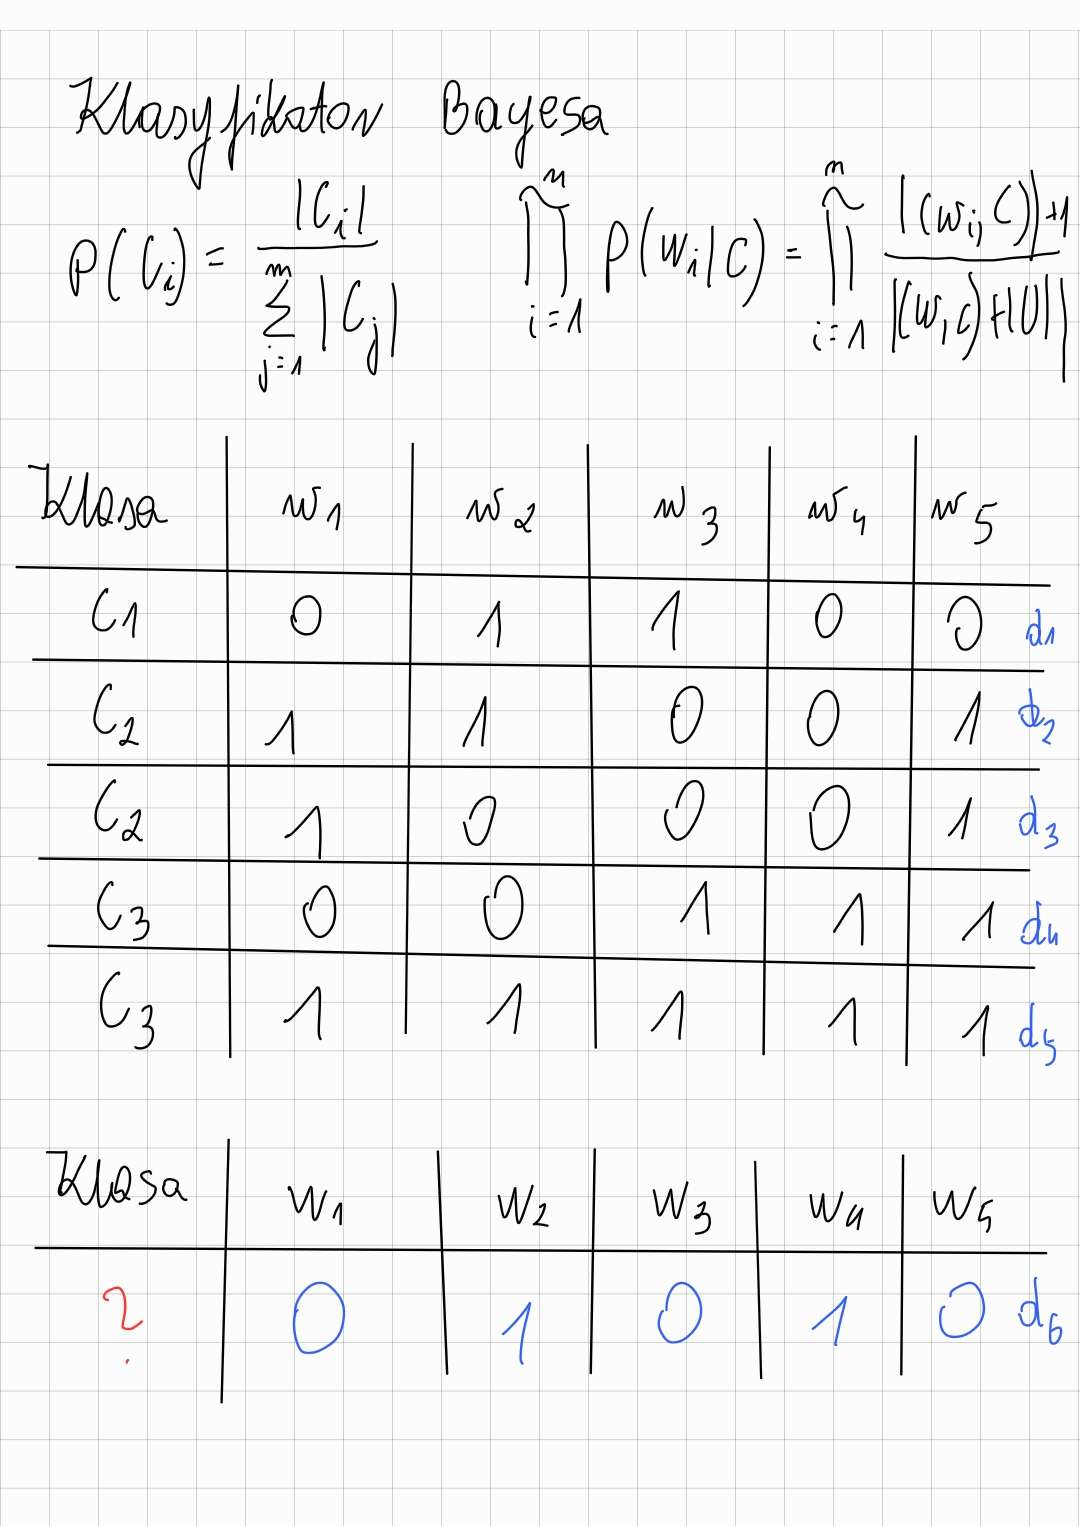
\includegraphics[width=0.75\textwidth]{bayes1.jpg}
\end{figure}

\newpage

Korzystając z twierdzenia Bayesa wyznaczamy najpierw
prawdopodobieństwa: 
\begin{itemize}
    \item wystąpienia każdej klasy $P(C_i)$
    \item wystąpienia każdej cechy w każdej klasie $P(w_j|C_i)$
\end{itemize}

Następnie wyznaczamy prawdopodobieństwa warunkowe $P(C_i|d_6)$,
i przypisujemy obserwację $d_6$ do klasy, dla której
prawdopodobieństwo warunkowe jest największe.

W tym przypadku obserwacja $d_6$ zostanie przypisana do klasy $C_3$.

\begin{figure}[H]
    \centering
    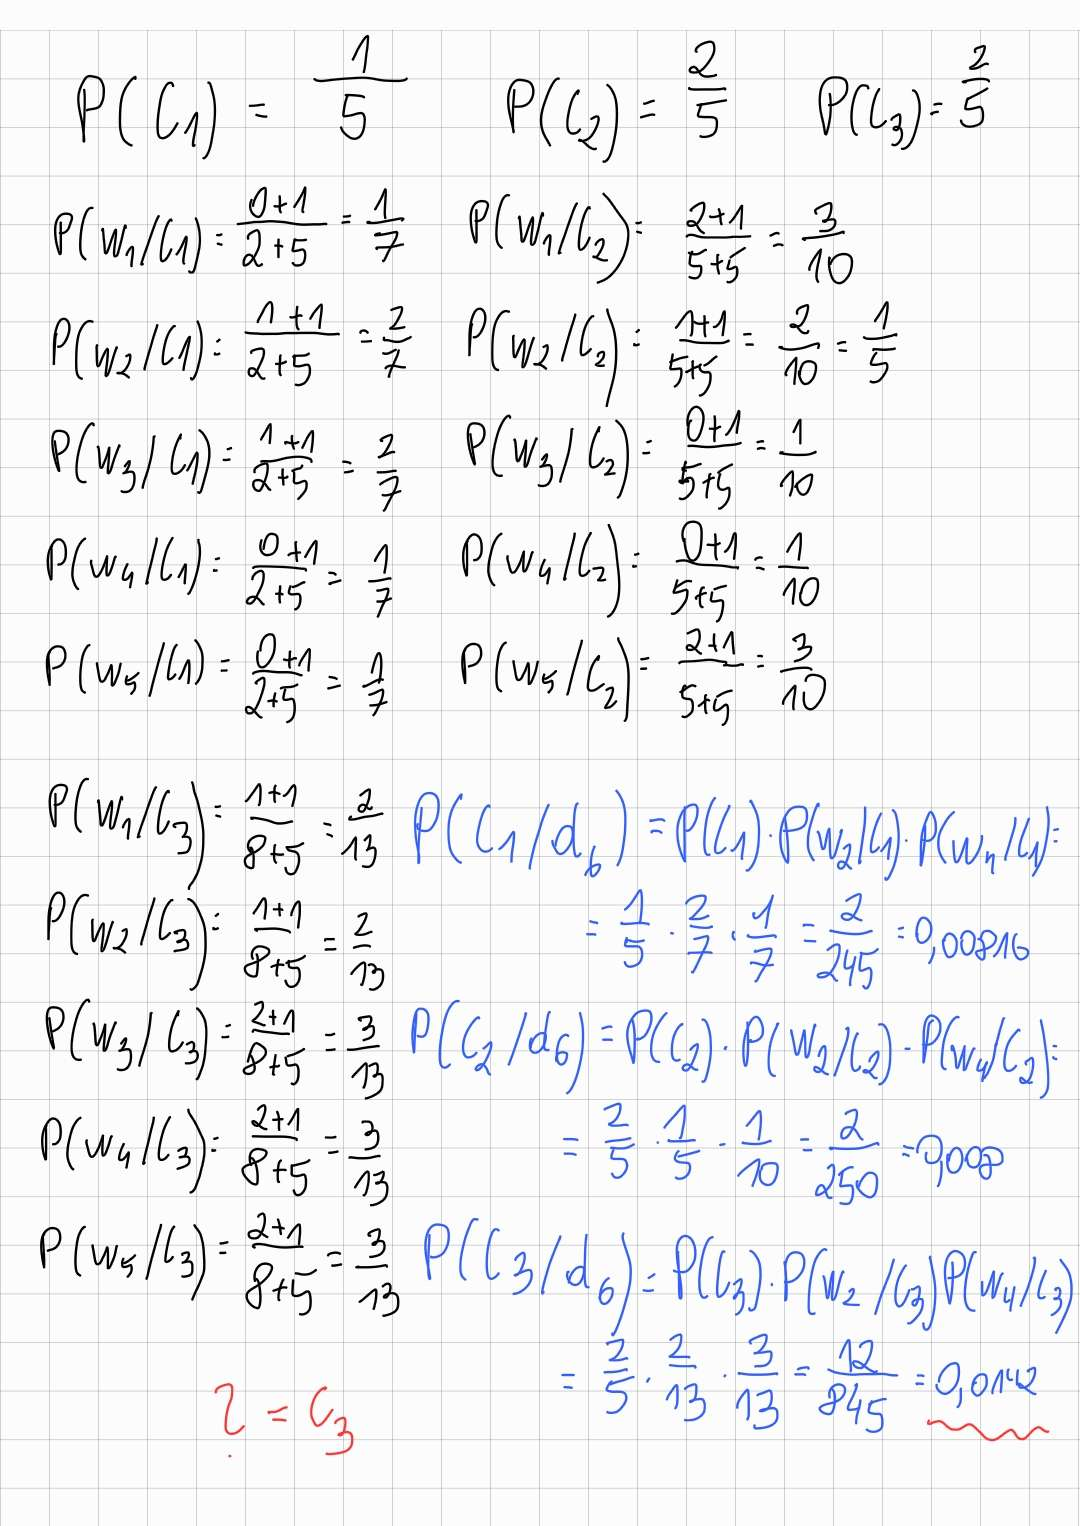
\includegraphics[width=0.75\textwidth]{bayes2.jpg}
\end{figure}

\newpage

\subsection{Klasyfikator K-NN}

Wybrałem następujące punkty obserwacji:
\begin{itemize}
    \item $d_1 = (1, 1)$ Klasa: $C_1$
    \item $d_2 = (-1, 2)$ Klasa: $C_1$
    \item $d_3 = (-2, -2)$ Klasa: $C_2$
    \item $d_4 = (2, -2)$ Klasa: $C_2$
    \item $d_5 = (\frac{1}{2}, -\frac{1}{2})$ Klasa: $C_2$
\end{itemize}

Zadaniem jest sklasyfikowanie obserwacji $d_6 = (-\frac{1}{2}, \frac{1}{2})$.
Za metrykę odległości przyjąłem metrykę euklidesową oraz $K=3$.

\begin{figure}[H]
    \centering
    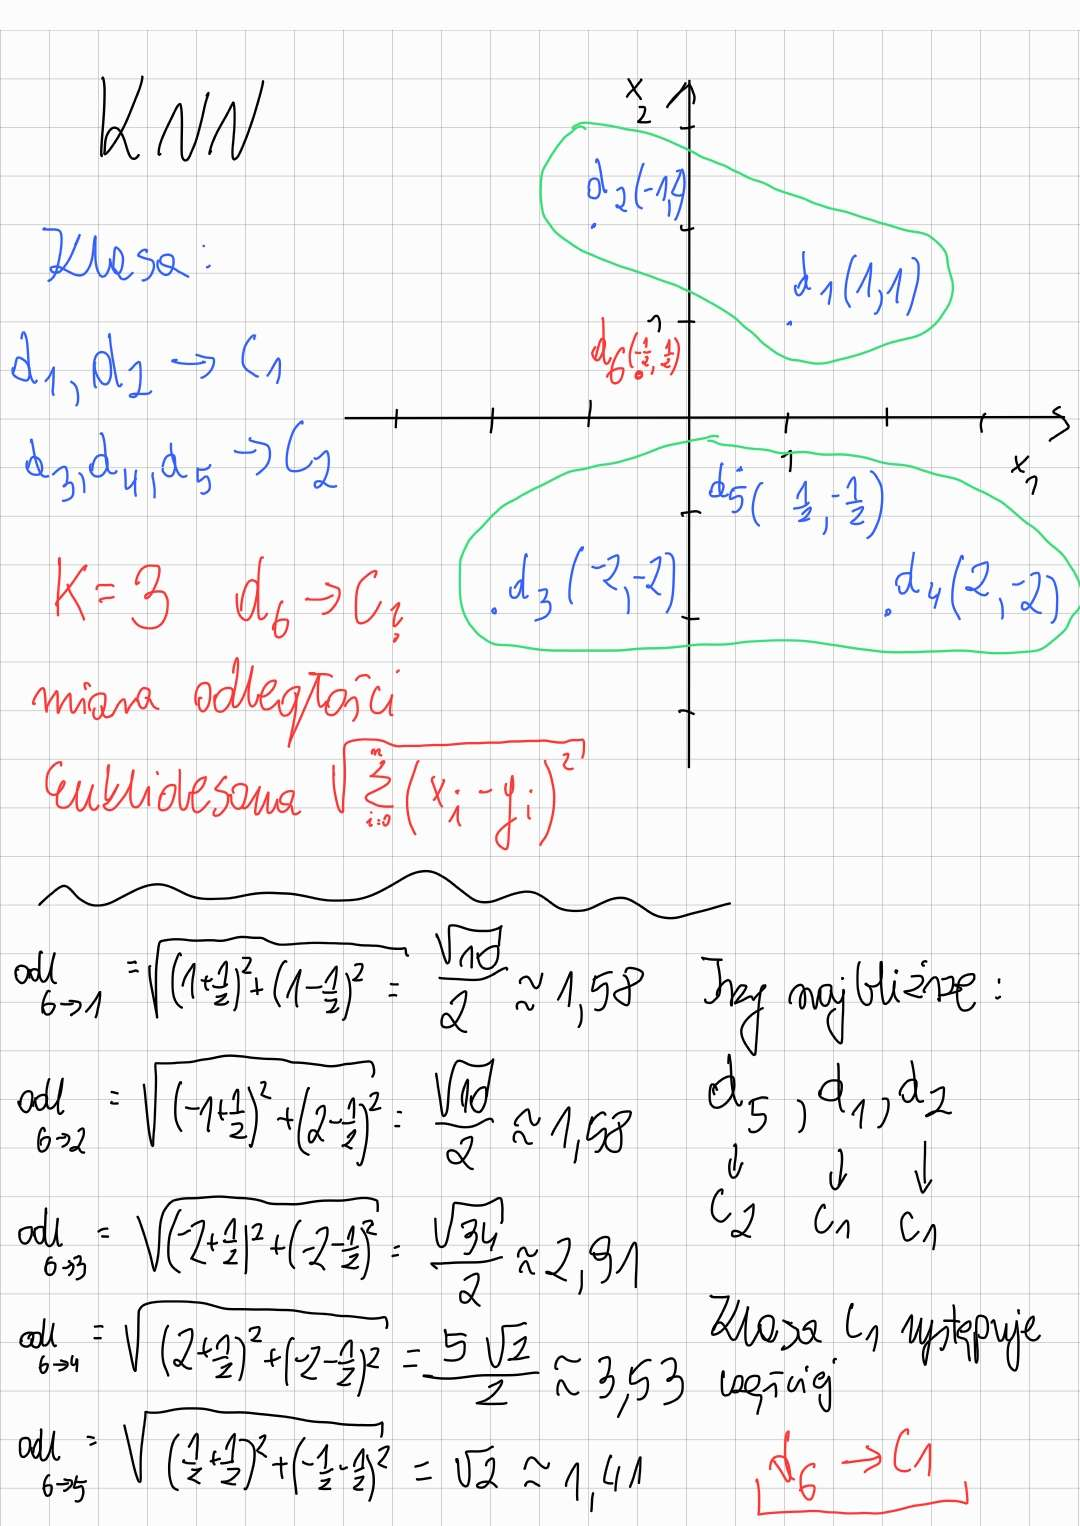
\includegraphics[width=0.75\textwidth]{knn.jpg}
\end{figure}

Według tego modelu obserwacja $d_6$ zostanie przypisana do klasy $C_1$.


\end{document}